\chapter{การทดสอบระบบ}
ขั้นตอนการทดสอบระบบงานถือเป็นขั้นตอนหนึ่งที่สำคัญของการสร้างระบบงานเนื่องจากเป็นการสรุปงานหรือเพื่อดูประสิทธิภาพของการพัฒนาระบบงานรวมทั้งทำให้ทราบถึงปัญหาที่อาจเกิดขึ้นก่อนที่จะนำระบบงานไปใช้งานจริง เพื่อทำการแก้ไขปัญหาได้ทันท่วงที ทั้งนี้เพื่อให้การพัฒนาระบบงานมีความสมบูรณ์มากที่สุด ทำให้เกิดประโยชน์ต่อผู้ใช้งาน และผู้พัฒนาระบบต่อไป แอปพลิเคชันค้นหายาเพื่อคุณที่ได้พัฒนาขึ้นนี้ 
ได้มีการทดสอบระบบงานในส่วนต่างๆ ดังนี้
\begin{itemize}[label={--}]
	\item ผลการทดสอบการค้นหายาแบบทั่วไป
	\item ผลการทดสอบการค้นหายาแบบขั้นสูง
	\item ผลการทดสอบเลือกดูรายละเอียดยา
	\item ผลการทดสอบถ่ายรูปภาพเพื่อการพิสูจน์เอกลักษณ์ยาเม็ด
	\item ผลการทดสอบการ rounting ของเว็บเซอร์วิส
\end{itemize}

\section{ผลการทดสอบการค้นหายาแบบทั่วไป}
% \begin{table}[H]
% 	\caption{ผลการทดสอบค้นหายาแบบทั่วไป}
% 	\label{tab:test1}
% 	\begin{tabular}{c}
% 		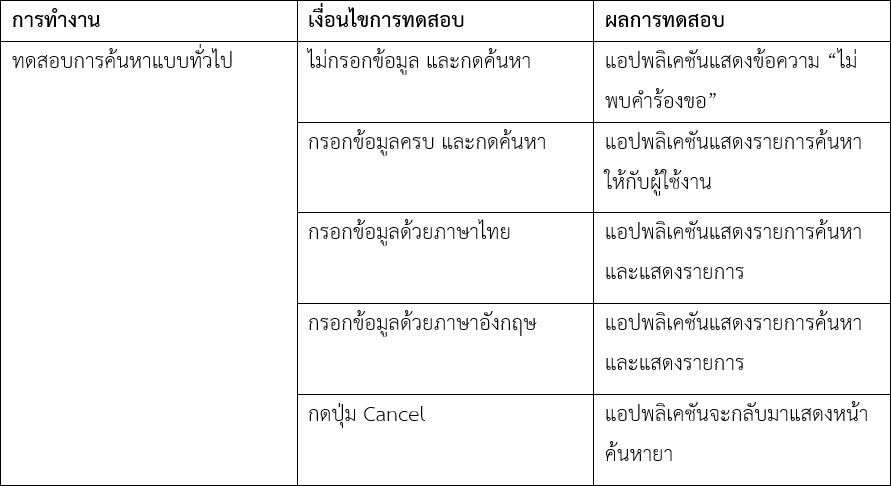
\includegraphics[width=\columnwidth]{Figures/table/test1}	\\ 
% 	\end{tabular}
% \end{table}
\begin{table}[H]
	\caption{ผลการทดสอบค้นหายาแบบทั่วไป}
    \centering	
	\label{tab:test1}
    \begin{tabular}{ | p{4.5cm} | p{4.5cm} | p{4.5cm} | }
    \hline
	% {\setstretch{1.0} } 
	การทำงาน & เงื่อนไขการทดสอบ & ผลการทดสอบ \\ \hline
	\setstretch{1.0}{ทดสอบการค้นหาแบบทั่วไป 
	& \setstretch{1.0}{ไม่กรอกข้อมูล และกดค้นหา }
	& \setstretch{1.0}{แอปพลิเคชันแสดงข้อความ “ไม่พบคำร้องขอ”} \\ \cline{2-3} 
	& \setstretch{1.0}{กรอกข้อมูลครบ และกดค้นหา} 
	& \setstretch{1.0}{แอปพลิเคชันแสดงรายการค้นหาให้กับผู้ใช้งาน} \\ \cline{2-3} 
	& \setstretch{1.0}{กรอกข้อมูลด้วยภาษาไทย}  
	& \setstretch{1.0}{แอปพลิเคชันแสดงรายการค้นหา และแสดงรายการ} \\ \cline{2-3} 
	& \setstretch{1.0}{กรอกข้อมูลด้วยภาษาอังกฤษ} 
	& \setstretch{1.0}{แอปพลิเคชันแสดงรายการค้นหา และแสดงรายการ} \\ \cline{2-3} 
	& \setstretch{1.0}{กดปุ่ม Cancel} 
	& \setstretch{1.0}{แอปพลิเคชันจะกลับมาแสดงหน้าค้นหายา} \\ \hline
    \end{tabular}
\end{table}


\section{ผลการทดสอบการค้นหายาแบบขั้นสูง}
% \begin{table}[H]
% 	\caption{ผลการทดสอบการค้นหายาแบบขั้นสูง}
% 	\label{tab:test2}
% 	\begin{tabular}{c}
% 		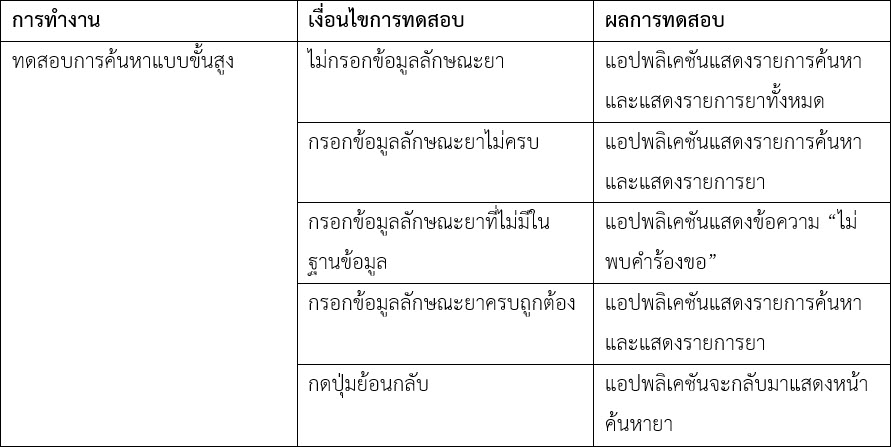
\includegraphics[width=\columnwidth]{Figures/table/test2}	\\ 
% 	\end{tabular}
% \end{table}
	\begin{table}[H]
		\caption{ผลการทดสอบการค้นหายาแบบขั้นสูง}
		\centering	
		\label{tab:test2}
		\begin{tabular}{ | p{4.5cm} | p{4.5cm} | p{4.5cm} | }
		\hline
		การทำงาน & เงื่อนไขการทดสอบ & ผลการทดสอบ \\ \hline
		\setstretch{1.0}{ทดสอบการค้นหาแบบขั้นสูง }
		& \setstretch{1.0}{ไม่กรอกข้อมูลลักษณะยา }
		& \setstretch{1.0}{แอปพลิเคชันแสดงข้อความ “ไม่พบคำร้องขอ”} \\ \cline{2-3} 
		& \setstretch{1.0}{กรอกข้อมูลลักษณะยาไม่ครบ }
		& \setstretch{1.0}{แอปพลิเคชันแสดงรายการค้นหา และแสดงรายการยา} \\ \cline{2-3} 
		& \setstretch{1.0}{กรอกข้อมูลลักษณะยาที่ไม่มีในฐานข้อมูล }
		& \setstretch{1.0}{แอปพลิเคชันแสดงข้อความ “ไม่พบคำร้องขอ”} \\ \cline{2-3} 
		& \setstretch{1.0}{กรอกข้อมูลลักษณะยาครบถูกต้อง }
		& \setstretch{1.0}{แอปพลิเคชันแสดงรายการค้นหา และแสดงรายการยา} \\ \cline{2-3} 
		& \setstretch{1.0}{กดปุ่มย้อนกลับ }
		& \setstretch{1.0}{แอปพลิเคชันจะกลับมาแสดงหน้าค้นหายา} \\ \hline
		\end{tabular}
	\end{table}


\section{ผลการทดสอบเลือกดูรายละเอียดยา}
% \begin{table}[H]
% 	\caption{ผลการทดสอบเลือกดูรายละเอียดยา}
% 	\label{tab:test3}
% 	\begin{tabular}{c}
% 		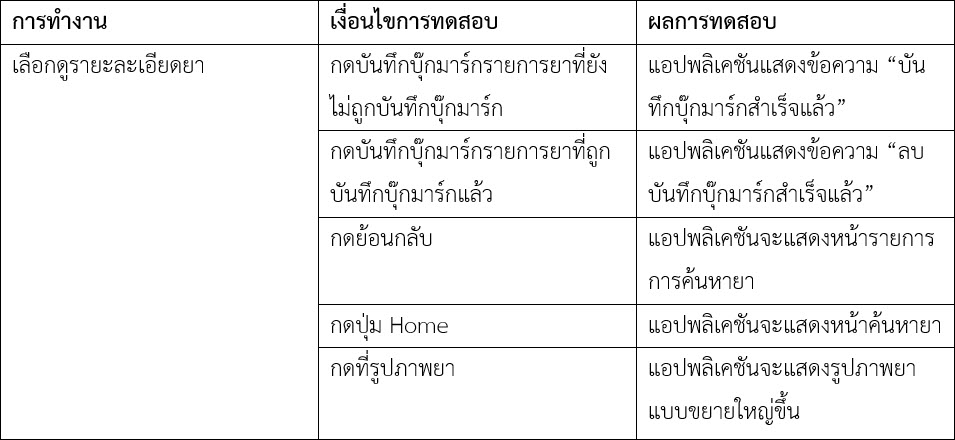
\includegraphics[width=\columnwidth]{Figures/table/test3}	\\ 
% 	\end{tabular}
% \end{table}
	\begin{table}[H]
		\caption{ผลการทดสอบเลือกดูรายละเอียดยา}
		\centering	
		\label{tab:test3}
		\begin{tabular}{ | p{4.5cm} | p{4.5cm} | p{4.5cm} | }
		\hline
		การทำงาน & เงื่อนไขการทดสอบ & ผลการทดสอบ \\ \hline
		\setstretch{1.0}{เลือกดูรายะละเอียดยา}
		& \setstretch{1.0}{กดบันทึกบุ๊กมาร์กรายการยาที่ยังไม่ถูกบันทึกบุ๊กมาร์ก} 
		& \setstretch{1.0}{แอปพลิเคชันแสดงข้อความ “บันทึกบุ๊กมาร์กสำเร็จแล้ว”} \\ \cline{2-3} 
		& \setstretch{1.0}{กดบันทึกบุ๊กมาร์กรายการยาที่ถูกบันทึกบุ๊กมาร์กแล้ว }
		& \setstretch{1.0}{แอปพลิเคชันแสดงข้อความ “ลบบันทึกบุ๊กมาร์กสำเร็จแล้ว”} \\ \cline{2-3} 
		& \setstretch{1.0}{กดย้อนกลับ }
		& \setstretch{1.0}{แอปพลิเคชันจะแสดงหน้ารายการการค้นหายา} \\ \cline{2-3} 
		& \setstretch{1.0}{กดปุ่ม Home }
		& \setstretch{1.0}{แอปพลิเคชันจะแสดงหน้าค้นหายา} \\ \cline{2-3} 
		& \setstretch{1.0}{กดที่รูปภาพยา }
		& \setstretch{1.0}{แอปพลิเคชันจะแสดงรูปภาพยาแบบขยายใหญ่ขึ้น} \\ \hline
		\end{tabular}
	\end{table}


\section{ผลการทดสอบถ่ายรูปภาพเพื่อการพิสูจน์เอกลักษณ์ยาเม็ด}
% \begin{table}[H]
% 	\caption{ผลการทดสอบถ่ายรูปภาพเพื่อการพิสูจน์เอกลักษณ์ยาเม็ด}
% 	\label{tab:test4}
% 	\begin{tabular}{c}
% 		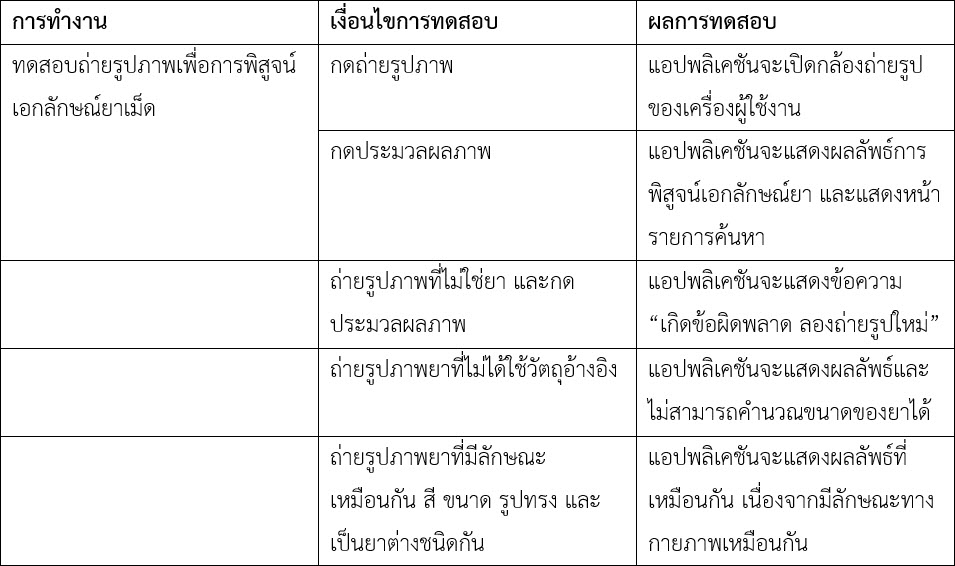
\includegraphics[width=\columnwidth]{Figures/table/test4}	\\ 
% 	\end{tabular}
% \end{table}
	\begin{table}[H]
		\caption{ผลการทดสอบถ่ายรูปภาพเพื่อการพิสูจน์เอกลักษณ์ยาเม็ด}
		\centering	
		\label{tab:test4}
		\begin{tabular}{ | p{4.5cm} | p{4.5cm} | p{4.5cm} | }
		\hline
		การทำงาน & เงื่อนไขการทดสอบ & ผลการทดสอบ \\ \hline
		\setstretch{1.0}{ทดสอบถ่ายรูปภาพเพื่อการพิสูจน์เอกลักษณ์ยาเม็ด}
		& \setstretch{1.0}{กดถ่ายรูปภาพ }
		& \setstretch{1.0}{แอปพลิเคชันจะเปิดกล้องถ่ายรูปของเครื่องผู้ใช้งาน} \\ \cline{2-3} 
		& \setstretch{1.0}{กดประมวลผลภาพ }
		& \setstretch{1.0}{แอปพลิเคชันจะแสดงผลลัพธ์การพิสูจน์เอกลักษณ์ยา และแสดงหน้ารายการค้นหา} \\ \cline{2-3} 
		& \setstretch{1.0}{ถ่ายรูปภาพที่ไม่ใช่ยา และกดประมวลผลภาพ }
		& \setstretch{1.0}{แอปพลิเคชันจะแสดงข้อความ “เกิดข้อผิดพลาด ลองถ่ายรูปใหม่”} \\ \cline{2-3} 
		& \setstretch{1.0}{ถ่ายรูปภาพยาที่ไม่ได้ใช้วัตถุอ้างอิง }
		& \setstretch{1.0}{แอปพลิเคชันจะแสดงผลลัพธ์และไม่สามารถคำนวณขนาดของยาได้} \\ \cline{2-3} 
		& \setstretch{1.0}{ถ่ายรูปภาพยาที่มีลักษณะเหมือนกัน สี ขนาด รูปทรง และเป็นยาต่างชนิดกัน} 
		& \setstretch{1.0}{แอปพลิเคชันจะแสดงผลลัพธ์ที่เหมือนกัน เนื่องจากมีลักษณะทางกายภาพเหมือนกัน} \\ \hline
		\end{tabular}
	\end{table}


\section{ผลการทดสอบการ rounting ของเว็บเซอร์วิส}
% \begin{table}[H]
% 	\caption{ผลการทดสอบการ rounting ของเว็บเซอร์วิส}
% 	\label{tab:test5}
% 	\begin{tabular}{c}
% 		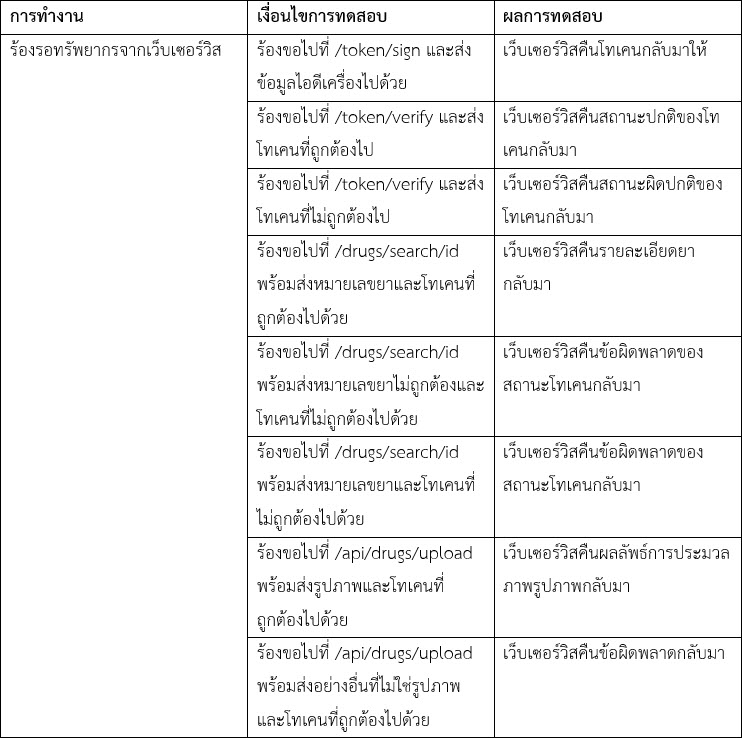
\includegraphics[width=\columnwidth]{Figures/table/test5}	\\ 
% 	\end{tabular}
% \end{table}
	\begin{table}[H]
		\caption{ผลการทดสอบการ rounting ของเว็บเซอร์วิส}
		\centering	
		\label{tab:test5}
		\begin{tabular}{ | p{4.5cm} | p{4.5cm} | p{4.5cm} | }
		\hline
		การทำงาน & เงื่อนไขการทดสอบ & ผลการทดสอบ \\ \hline
		\setstretch{1}{ร้องรอทรัพยากรจากเว็บเซอร์วิส}
		& \setstretch{1} {ร้องขอไปที่ /token/sign และส่งข้อมูลไอดีเครื่องไปด้วย}
		& \setstretch{1} {เว็บเซอร์วิสคืนโทเคนกลับมาให้} \\ \cline{2-3} 
		& \setstretch{1} {ร้องขอไปที่ /token/sign และไม่ส่งข้อมูลไอดีเครื่องไปด้วย} 
		& \setstretch{1} {เว็บเซอร์วิสคืนโทเคนกลับมาให้} \\ \cline{2-3} 
		& \setstretch{1} {ร้องขอไปที่ /token/verify และส่งโทเคนที่ถูกต้องไป} 
		& \setstretch{1} {เว็บเซอร์วิสคืนสถานะปกติของโทเคนกลับมา} \\ \cline{2-3} 
		& \setstretch{1} {ร้องขอไปที่ /token/verify และส่งโทเคนที่ไม่ถูกต้องไป} 
		& \setstretch{1} {เว็บเซอร์วิสคืนสถานะผิดปกติของโทเคนกลับมา} \\ \cline{2-3} 
		& \setstretch{1} {ร้องขอไปที่ /token/verify และไม่ส่งโทเคนไปด้วย} 
		& \setstretch{1} {เว็บเซอร์วิสคืนสถานะผิดปกติของโทเคนกลับมา} \\ \cline{2-3} 
		& \setstretch{1} {ร้องขอไปที่ /drugs/search/id พร้อมส่งหมายเลขยาและโทเคนที่ถูกต้องไปด้วย} 
		& \setstretch{1} {เว็บเซอร์วิสคืนรายละเอียดยากลับมา} \\ \cline{2-3} 
		& \setstretch{1} {ร้องขอไปที่ /drugs/search/id พร้อมส่งหมายเลขยาไม่ถูกต้องและโทเคนที่ไม่ถูกต้องไปด้วย} 
		& \setstretch{1} {เว็บเซอร์วิสคืนข้อผิดพลาดของสถานะโทเคนกลับมา} \\ \cline{2-3} 
		& \setstretch{1} {ร้องขอไปที่ /drugs/search/id พร้อมส่งหมายเลขยาและโทเคนที่ไม่ถูกต้องไปด้วย}
		& \setstretch{1} {เว็บเซอร์วิสคืนข้อผิดพลาดของสถานะโทเคนกลับมา} \\ \cline{2-3} 
		& \setstretch{1} {ร้องขอไปที่ /api/drugs/upload พร้อมส่งรูปภาพและโทเคนที่ถูกต้องไปด้วย} 
		& \setstretch{1} {เว็บเซอร์วิสคืนผลลัพธ์การประมวลภาพรูปภาพกลับมา} \\ \cline{2-3} 
		& \setstretch{1} {ร้องขอไปที่ /api/drugs/upload พร้อมส่งไฟล์ที่ไม่ใช่รูปภาพและโทเคนที่ถูกต้องไปด้วย}
		& \setstretch{1} {เว็บเซอร์วิสคืนข้อผิดพลาดกลับมา} \\ \hline
		\end{tabular}
	\end{table}

